\documentclass[a4paper]{article}
\usepackage[left=1.5cm,right=2cm,top=2cm,bottom=1.5cm]{geometry}
\usepackage{graphicx} % Required for inserting images
\usepackage{physics}
\usepackage{pgfplots}
\usepackage{amsthm}
\title{Second-order phase transition through mean-field approach}
\author{Vo Chau Duc Phuong $^1$}
\date{$^1$the Abdus Salam International Center for Theoretical Physics\vspace{4pt}\\March 2025}
\pgfplotsset{
	compat=1.12,
	/pgf/declare function={
		L(\x) = 1./tanh(x) - 1./x;
		B(\n,\x) = (1.+1./(2.*\n))*1/tanh((1.+1./(2.*\n))*x) - 1/(2*\n)*1/tanh(x/(2.*\n));
	},
}

\begin{document}
	\maketitle
	\begin{abstract}
Using the mean-field approach, I will show two way to calculate and model a second-phase transition system from partition function and linking them together with the classical limit and also showing the equivalent between both in Landau theory.
	\end{abstract}
\section{Missionary Expected Value:} %segg jo kè
	\subsection{Semi-classical approach}
\quad An independence particle placed inside a magnetic field \(\vec{H}\) will have the single-body Hamiltonian, which is equivalent with the many-body electrons system in the independence particle approximation:
	\begin{equation}
		\mathcal{H} = - \vec{M} \cdot \vec{H}.
	\end{equation}
\quad Choosing the convention for the magnetic field \(\textbf{H}\) will be placed along the z axis, the Hamiltonian should be express in the sphere coordinate:
	\begin{equation}
		\mathcal{H} = - m_z.H = -mH . \cos \theta.
	\end{equation}
\quad Therefore, we can calculate the canonical partition function for an electron:
	\begin{equation}
		Z = \int e^{-\beta \mathcal{H}} d\Omega.
	\end{equation}
\quad In this equation, the integral over radius \(r\) will be neglect since the total moment \(m\) is constant for a particle. Therefore:
	\begin{equation}
		Z = 2\pi \int_{0}^\pi e^{\beta m H \cos \theta } \sin \theta d\theta= 2\pi \int_{-1}^{1} e^{\beta m H x} dx = 4\pi \frac{sinh(\beta m H)}{\beta m H}.
	\end{equation}
\quad In the canonical, the average value of magnetic moment along z  \(m_z\) axis can be calculated through:
	\begin{align}
		\ev{m_Z} =& \frac{1}{Z} \int m_z e^{\beta H m_z} = \frac{\partial_{\beta H}Z}{Z}\\
		=& -\frac{1}{(\beta H)} + m\coth\beta m H = m L(\beta m H),
	\end{align}
	in which the \(L(x)\) is the Langevin function:
	\begin{equation}
		L(x) = \coth x - \frac{1}{x}
	\end{equation}
\quad The second phase-transition however, come from the idea that the self interaction between the particle inside the system make the magnetic momentum when into two energy minimize states, all up or all down. We will including the mean-field approximation through the total field:
\begin{equation}
	H \to H_{total}  = H_{ext} + \Gamma \ev{m_z},
\end{equation}
with the \(\Gamma\) acting as a phenomenon parameter. These approach will give us the self consistent equation:
\begin{equation}
	\ev{m_z} = m L(\beta m (H_{ext} + \Gamma \ev{m_z}))
\end{equation}
The transition can appear without the external field, therefore \(H_{ext} \to 0\) give us:
\begin{equation}
	\ev{m_z} = m L(\beta m \Gamma \ev{m_z})
\end{equation}
The second-order phase transition happens when \(\ev{m_z} \to 0\) at \(T \to T_c\), therefore allow us to approximate the Langevin function to the first order of the limit \(x \ll 1\):
\begin{equation}
	L(x\ll 1) = \frac{1}{x} + \frac{x}{3} +O(x^3) - \frac{1}{x} \approx \frac{x}{3},
\end{equation}
give us:
\begin{align}
	\ev{m_z} =& \frac{m^2 \beta \Gamma \ev{m_z}}{3}\nonumber\\
	k_B T_c  =& \frac{m^2 \Gamma}{3},
\end{align}
and when we consider a higher expansion on the Langevin function:
\begin{align}
	\ev{m_z}\frac{\beta m \Gamma}{m^2} =& \frac{x}{3} - \frac{x^3}{45} \nonumber\\
	\frac{T}{T_c} =& 1 - \frac{z^2}{15} \nonumber\\
	\Rightarrow z =& \pm \sqrt{15\Gamma k_B m (T_c-T)} = \pm z_0.
\end{align}
\quad This expression give us two states that can happens when the \(T < T_c\), we neglect the trivial \(\ev{m_z} = 0\) in the previous calculation due to the unstable of this point in compare with the stable points \(z_0\). From the Langevin function, we also can derive Curie's law:
\begin{align}
	\ev{m_z} \approx& \frac{m^2 H}{3 k_B T} \nonumber\\
	\chi_ 0 =& \frac{N}{V} \lim_{H \to 0} \frac{M_z}{H} = \frac{n_0 m^2}{3k_B T} \equiv \frac{C}{T}\quad \text{(Q.E.D)}
\end{align}
Curie law is derived in assumption that the spin will not "talk" (interact) to other spins in the system. In contract, we can use the same mean-field approach to derive the Curie-Weiss law:
\begin{align}
	\ev{m_z} \approx& \frac{m^2 H_{ext}}{3k_B T} + \frac{m^2 \Gamma \ev{m_z}}{3T} = \frac{m^2 H_{ext}}{3k_B T} + \frac{T_c\ev{m_z}}{T}\nonumber\\
	\chi =& \frac{N}{V} \lim_{H_{ext} \to 0} \frac{m^2}{3k_B T} + \frac{T_c N}{T V}\lim_{H_{ext} \to 0} \frac{\ev{m_z}}{H_{ext}} = \chi_0 + \chi \frac{T_c}{T}\nonumber\\
	\Rightarrow \chi =& \frac{\chi_0}{1-\frac{T_c}{T}} \equiv \frac{C}{T - T_c} \quad \text{(Q.E.D)}
\end{align} 
\subsection{Quantum Approach}
\quad The same approach can be used but the angular momentum along the z direction will be quantized. In this case, it should be best to considering the picture that a whole particle will have the total angular momentum compose of angular momentum \(\vec{L}\) and spin \(\vec{S}\):
\begin{equation}
	\vec{J} = \vec{S} + \vec{L}.
\end{equation}
\quad The same degeneracy of the angular- and spin-momentum for these momenta give total degeneracy of \(2J + 1\) for \(m_j \in [-J,J]\). In this scenario, we will expressing the interaction between the total momentum \(J\) and field \(H\):
\begin{align}
	\mathcal{H} =& - \vec{M}\cdot\vec{H}\\
	\vec{M} =& g_J \mu_B \vec{J},
\end{align}
in which \(g_J\) is the Landé factor define as\footnote{The definition above actually a pretty good approximation, the full expression can be derived from the perturbation theory}:
\begin{equation}
	g_J = 1 + \frac{J(J+1) + S(S+1) - L(L+1)}{2J(J+1)}.
\end{equation}
\quad Partition function is:
\begin{align}
	Z_J =& \sum_{m = -J}^{J} e^{\beta g_J \mu_B H m} = e^{ - \beta g_J \mu_B H J} + e^{ - \beta g_J \mu_B H (J-1)} + ... + e^{\beta g_J \mu_B H J}\nonumber\\
	=& e^{ - \beta g_J \mu_B H J} (1 + e^{ \beta g_J \mu_B H} + e^{ 2\beta g_J \mu_B H} + ... + e^{ 2\beta g_J \mu_B H J})\nonumber\\
	=& e^{ - \beta g_J \mu_B H J} \frac{1 - e^{\beta g_J \mu_B H(2J + 1)}}{1 - e^{\beta g_J \mu_B H}} = \frac{e^{ - \beta g_J \mu_B H J} - e^{\beta g_J \mu_B H(J+1)}}{1 - e^{\beta g_J \mu_B H}} \nonumber\\
	=& \frac{e^{ - \beta g_J \mu_B H (J + 1/2)} - e^{\beta g_J \mu_B H(J + 1/2)}}{e^{-\beta g_J \mu_B H/2} - e^{\beta g_J \mu_B H/2}} = \frac{\sinh(\beta g_J \mu_B H (J + 1/2))}{\sinh(\beta g_J \mu_B H/2)}
\end{align}
\quad From this generalize partition function, we can recover the familiar partition function for the electron case \(J = S = \frac{1}{2}\):
\begin{equation}
	Z_{1/2} = \frac{\sinh ( g_{1/2}\beta  \mu_B H)}{\sinh ( g_{1/2}\beta \mu_B H/2)} = \frac{2\sinh ( g_{1/2}\beta \mu_B H/2) \cosh ( g_{1/2}\beta \mu_B H/2)}{\sinh ( g_{1/2}\beta \mu_B H/2)} = 2 \cosh ( \frac{g_{1/2}\beta \mu_B H}{2})
\end{equation}
Which in turn give us the expected value both generalize and spin \(1/2\) case:
\begin{align}
\ev{J_z} =& \frac{1}{Z}\sum_{m = -J}^{J} m e^{g_J \mu_B H m} = \frac{1}{Z g_{J}\mu_B H} \pdv{Z}{\beta}\nonumber\\ 
=& \bigg(J + \frac{1}{2}\bigg) \coth \bigg(\beta g_J \mu_B H \bigg(J + \frac{1}{2}\bigg)\bigg) - \frac{1}{2}\coth \bigg(\frac{\beta g_J \mu_B H}{2}\bigg)\nonumber \\
=& J \bigg[\bigg(1 + \frac{1}{2J}\bigg) \coth \bigg(y \bigg(1 + \frac{1}{2J}\bigg)\bigg) - \frac{1}{2J}\coth \bigg(\frac{y}{2J}\bigg)\bigg] = J B_{J}(y), \qquad y = \frac{\beta g_J \mu_B H}{2J},
\end{align}
in which \(B_J(y)\) is the Brillouin function, which defined as:
\begin{equation}
	B_J(y) = \bigg(1 + \frac{1}{2J}\bigg) \coth\bigg(y\bigg(1 + \frac{1}{2J}\bigg)\bigg) - \frac{1}{2J} \coth \frac{y}{2J}
\end{equation}
\begin{figure}[!ht]
\begin{center}
	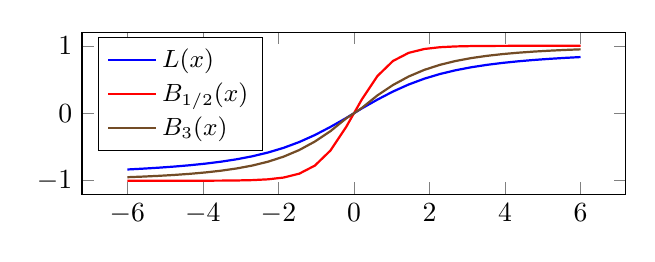
\begin{tikzpicture}
		\begin{axis}[legend style={font=\small},
			legend cell align=left,       % <---
			legend pos=north west,width=0.7\textwidth,
			height=0.3\textwidth,no markers,samples=30,y domain=-1.2:1.2]
			% ... and use it here
			\addplot+ [thick, domain=-6:6] {L(x)};
			\addplot+ [thick, domain=-6:6] {B(1./2,x)};
			\addplot+ [thick, domain=-6:6] {B(3.,x)};
			\legend{$L(x)$,$B_{1/2}(x)$,$B_{3}(x)$}
		\end{axis}
	\end{tikzpicture}
\caption{Brillouin's and Langevin's functions on the same graph}
\label{Fig: L and B}
\end{center}
\end{figure}
\quad As shown in Fig. \ref{Fig: L and B}, the Brillouin's function \(B_J (x)\)will converge to Langevin's \(L(x)\) function as \(J \to \infty\).
\begin{proof}
	\begin{align*}
		B_J(y) =& \bigg(1 + \frac{1}{2J}\bigg) \coth\bigg(y\bigg(1 + \frac{1}{2J}\bigg)\bigg) - \frac{1}{2J} \coth \frac{y}{2J}\\
		&\xrightarrow{J \to \infty} \coth (y) - \lim_{J\to \infty}\frac{1}{2J} \bigg(\frac{2J}{y} + \frac{y}{2J} + ...\bigg) = \coth (y) - \frac{1}{y} = L(y).\end{align*}
Therefore, at classical limit \(J \to \infty, B_{J}(y) \to L(y)\)
\end{proof}
For the electron \(S = 1/2\), we recover the usual relation:
\begin{align*}
	B_{1/2}(y) &= 2\coth(2y) - \coth(y) = \frac{1 + \tanh^2 (y) }{\tanh(y)} - \frac{1}{\tanh(y)} = tanh(y) \\
	\ev{J_z} &= J B_{J}(\beta g_J \mu_B H /2J) = \frac{1}{2} \tanh (\beta g_{1/2} \mu_B H)	
\end{align*}
The phase transition relation can be achieved by using the mean-field approach for the total field \(H\), through the self-consistence equation:
\begin{equation}
	\ev{M_z} = g_J \mu_B J B_{J}(\beta g_{1/2} \mu_B \big(H_{ext} + \Gamma \ev{M_z} \big)) \xrightarrow{H_{ext}} g_J \mu_B J B_{J}(\beta g_{1/2} \mu_B\Gamma \ev{M_z})
\end{equation}
At the transition point \(\ev{M_z} \to 0\), we can approximate the \(B_{\nu}(y) \approx \frac{y}{3} \frac{J + 1}{J}\):
\begin{align}
	\ev{M_z} =& g_J \mu_B J \beta g_{J} \mu_B J\frac{H_{ext} + \Gamma \ev{M_z}}{3} \frac{J + 1}{J}\nonumber\\
	\xrightarrow{H_{ext} \to 0}k_B T_c =&  (g_J \mu_B)^2 J\frac{J + 1}{3} \Gamma
\end{align}
\quad The \(J^2\) term in the equation give the idea of corresponding with the \(m^2\) term in semi-classical ansatz, in which \(J^2 \gg J\). Which the same proceed, Curie's law and Curie-Weiss's law can easily computed without and with mean-field approach, respectively:
\begin{equation}
	\chi_0 = \frac{N}{V}\lim_{H_{ext} \to 0} \frac{\ev{M_z}}{H_{ext}} = n\frac{g_J^2 \mu_B^2 }{3k_B T} \frac{J+1}{J} = \frac{C}{T}
\end{equation}
\begin{align*}
	\chi &= \frac{N}{V} \lim_{H_{ext} \to 0} \frac{\ev{M_z}}{H_{ext}} = \chi_0 + \frac{T_c}{T} \chi\\
	\Rightarrow \chi(T) &= \frac{\chi_0}{T - T_c}
\end{align*}

\end{document}
